\Variant{24.05.2025 (2-smena)}
\QQ{1}{Agar $a$, $b$ raqamlar uçun $5a+\dfrac5{11}b=45$ tenglik örinli bölsa, $2a+b$ ni toping.
\Opts{$24$}{$18$}{$36$}{$17$}}
\QQ{2}{Aytaylik
\[x=1+4+7+\dots+301,\qquad y=2+8+14+\dots+602\]
bölsin. Unday bölsa $\dfrac{y+2022x}x$ ni hisoblang.
\Opts{$2024$}{$2022$}{$2023$}{$2025$}}
\QQ{3}{Velosipedçi ikki şahar orasidagi masofani $4$ soatda bosib ötadi. Piyoda $12$ soatda bosib ötadi. Agar ikkalasi bir-biriga qarab harakatlansa neça soatdan keyin uçraşadi?
\Opts{$4$}{$2{,}5$}{$3$}{$2$}}
\QQ{4}{Agar uçta bir xil köylak narxi ikkita bir xil şim narxining $90$ foiziga teng bölsa, bir köylak narxi bir şim narxining neça foizini taşkil qiladi?
\Opts{$50$}{$70$}{$60$}{$65$}}
\QQ{5}{Quyidagi ifodaning qiymati qaysi oraliqda:
\[\frac1{\sqrt4+\sqrt3}+\frac1{\sqrt5+\sqrt4}+\dots+\frac1{\sqrt{25}+\sqrt{24}}\]
\Opts{$(2;\,3)$}{$[3;\,4)$}{$(1;\,2)$}{$(4;\,5)$}}
\QQ{6}{Hisoblang:
\[\frac4{\sqrt{13}+3}-\frac9{\sqrt{13}-2}\]
\Opts{$5$}{$-5$}{$-2\sqrt{13}$}{$2\sqrt{13}$}}
\QQ{7}{Ösuvçi geometrik progressiyada birinçi va törtinçi hadlari yiğindisi $70$ ga, ikkinçi va uçinçi hadlari yiğindisi $60$ ga teng bölsa, beşinçi hadni toping.
\Opts{$108$}{$71$}{$81$}{$67$}}
\QQ{8}{Arifmetik progressiyaning birinçi hadi $124$ ga teng va ayirmasi $-3\dfrac13$ bölsa, progressiyaning neçta hadi natural son böladi?
\Opts{$11$}{$13$}{$17$}{$15$}}
\QQ{9}{Hisoblang:
\[\frac{\left(2^3\right)^5\cdot5^{10}\cdot2}{10^8}-\frac{2^3\cdot2^3\cdot5^4\cdot5^2}{10^6}\]
\Opts{$6399$}{$100$}{$99$}{$200$}}
\QQ{10}{Ifodani soddalaştiring:
\[\frac{a^4-64}{a^2+8}-\frac{a^6-512}{a^4+8a^2+64}\]
\Opts{$a-b$}{$1$}{$a+b$}{$0$}}
\QQ{11}{Hisoblang:
\[\tg\left(\arcsin\left(-\frac12\right)\right)\]
\Opts{$-\sqrt3$}{$\sqrt3$}{$-\dfrac1{\sqrt3}$}{$\dfrac1{\sqrt3}$}}
\QQ{12}{Hisoblang:
\[\frac{\sqrt5-\sqrt3}{\sqrt7-\sqrt5-\sqrt3+1}+\frac{\sqrt3-\sqrt5}{\sqrt7+\sqrt5+\sqrt3+1}\]
\Opts{$\dfrac{\sqrt{15}+\sqrt7}4$}{$\dfrac{\sqrt{15}-\sqrt7}4$}{$-\dfrac{\sqrt{15}+\sqrt7}4$}{$\dfrac{\sqrt7-\sqrt{15}}4$}}
\QQ{13}{Tenglik örinli böladigan $a$ ning qiymatini toping.
\[(\sin4x+\cos4x)\left(\sin^34x-\cos^34x\right)=\frac14\sin ax-\cos8x\]
\Opts{$16$}{$8$}{$-8$}{$-16$}}
\QQ{14}{$|2x+3|<15$ tengsizlikning neçta butun yeçimi bor?
\Opts{$12$}{$15$}{$17$}{$14$}}
\QQ{15}{$\dfrac{5x-\lg0{,}1}{\sqrt2-\sqrt[3]3}<0$ tengsizlik $[-10;\,20]$ oraliqda neçta butun yeçimga ega?
\Opts{$17$}{$19$}{$20$}{$21$}}
\QQ{16}{Tenglamalar sistemasi neçta yeçimga ega?
\[\begin{cases}\log_xy+\log_yx=2,\\ x^2-y=30\end{cases}\]
\Opts{$1$}{$2$}{$3$}{$0$}}
\QQ{17}{Tenglamaning haqiqiy ildizlari yiğindisini toping.
\[\sqrt[3]{36-12x+x^2}+\sqrt[3]{x^2+6x+9}-\sqrt[3]{18+3x-x^2}=3\]
\Opts{$5$}{$7$}{$-2$}{$3$}}
\QQ{18}{$25\cdot2^x-10^x+5^x\ge25$ tengsizlikni qanoatlantiruvçi butun sonlar yiğindisini toping.
\Opts{$2$}{$3$}{$5$}{$6$}}
\QQ{19}{$x\left(x^2-2x+4\right)=2x+1$ tenglama neçta haqiqiy ildizga ega?
\Opts{$3$}{$2$}{$1$}{$0$}}
\QQ{20}{$f(x)=\sqrt3x+2$ va $g(x)=\dfrac1{\sqrt3}x+3$ funksiya grafiklari berilgan bölsa, ular orasidagi $a$ burçakni toping.
\qfig{\begin{tikzpicture}[scale=0.9,font=\small]
\draw[-{Stealth[length=4pt]}] (-2,0)--(3.2,0) node[right] {$x$}; \draw[-{Stealth[length=4pt]}] (0,-0.8)--(0,5.5) node[left] {$y$};
\draw (-1.6,-0.771)--(1.8,5.118); \draw (-2,1.845)--(3,4.732);
\draw (0.866,3.5)+(210:0.55) arc (210:240:0.55); \node at (0.45,2.95) {\scriptsize$a$};
\node[left] at (1.6,5.2) {$f(x)=\sqrt3x+2$}; \node[right] at (3,4.732) {$g(x)=\frac1{\sqrt3}x+3$}; \node[below left] at (0,0) {$O$};
\end{tikzpicture}}
\Opts{$45^\circ$}{$30^\circ$}{$60^\circ$}{$90^\circ$}}
\QQ{21}{$f(x)=\dfrac{x^2-x}2$ va $g(x)=\dfrac{x-x^2}2$ bölsa, $f(x+1)+g(1-x)=x^3$ tenglamaning ildizlari yiğindisini toping.
\Opts{$2$}{$-1$}{$1$}{$0$}}
\QQ{22}{$f(x)=\left|\ln x-\log_{\sin x}\cos x\right|$ bölsa, $f'\left(\dfrac\pi4\right)$ ni toping.
\Opts{$4\left(\log_2e-\dfrac1\pi\right)$}{$-4\left(\log_2e-\dfrac1\pi\right)$}{$4\left(\log_2e+\dfrac1\pi\right)$}{$-4\left(\log_2e+\dfrac1\pi\right)$}}
\QQ{23}{$f(x)=\dfrac2{\sqrt{2-x^2}}$ funksiyaning $(-1;\,0)$ nuqtadan ötuvçi boşlanğiç funksiyasini toping.
\Opts{$2\arcsin\dfrac x{\sqrt2}+\pi$}{$2\arcsin\dfrac x2-\pi$}{$2\arcsin\dfrac x{\sqrt2}+\dfrac\pi2$}{$2\arcsin\dfrac x{\sqrt2}-\dfrac\pi2$}}
\QQ{24}{Tomoni $1$ ga teng bölgan $11$ ta kvadrat va kvadrat uçlarida yotgan $4$ ta nuqta berilgan. Böyalgan soha yuzini toping.
\qfig{\begin{tikzpicture}[scale=0.85,font=\small]
\fill[qfill] (1,4)--(5,0)--(0,1)--(2,1)--cycle;
\draw (0,0) grid (5,1); \draw (1,1) grid (4,2); \draw (1,2) grid (3,3); \draw (1,3) grid (2,4);
\draw (1,4)--(5,0)--(0,1)--(2,1)--cycle;
\foreach \p in {(1,4),(5,0),(0,1),(2,1)} \fill \p circle (2.5pt);
\end{tikzpicture}}
\Opts{$5$}{$4$}{$10$}{$8$}}
\QQ{25}{$ABC$ va $BDC$ töğri burçakli uçburçaklar ($\angle C=\angle B=90^\circ$) berilgan. $|AC|=|CB|$, $\angle CDB=30^\circ$ va gipotenuzalar $E$ nuqtada kesişsa, $BED$ uçburçak yuzining $ABC$ uçburçak yuziga nisbatini toping.
\qfig{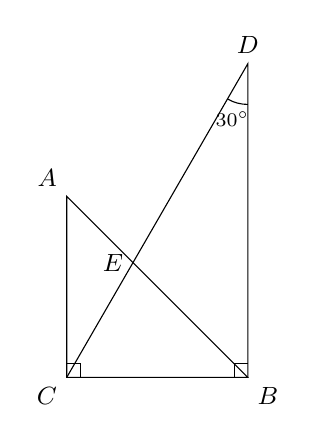
\begin{tikzpicture}[scale=1.15,font=\small]
\coordinate (C) at (0,0); \coordinate (B) at (2,0); \coordinate (A) at (0,2); \coordinate (D) at (2,3.464); \coordinate (E) at (0.732,1.268);
\draw (A)--(C)--(B)--cycle; \draw (C)--(D)--(B);
\draw (0,0.15)--(0.15,0.15)--(0.15,0); \draw (2,0.15)--(1.85,0.15)--(1.85,0);
\draw (D)+(240:0.45) arc (240:270:0.45); \node at (1.83,2.85) {\scriptsize$30^\circ$};
\node[below left] at (C) {$C$}; \node[below right] at (B) {$B$}; \node[above left] at (A) {$A$}; \node[above] at (D) {$D$}; \node[left] at (E) {$E$};
\end{tikzpicture}}
\Opts{$\dfrac{3\sqrt3-3}2$}{$\dfrac{3-\sqrt3}2$}{$\dfrac{3\sqrt3+3}2$}{$\dfrac{\sqrt3+3}2$}}
\QQ{26}{$ABC$ — töğri burçakli uçburçak ($\angle C=90^\circ$). $AD=4$, $CD=6$, $DE=EB=5$ bölsa, ştrixlangan yuzani toping.
\qfig{\begin{tikzpicture}[scale=0.34,font=\small]
\coordinate (C) at (0,0); \coordinate (A) at (10,0); \coordinate (D) at (6,0); \coordinate (B) at (0,8); \coordinate (E) at (3,4);
\fill[qfill] (B)--(E)--(A)--cycle;
\draw (A)--(B)--(C)--cycle; \draw (B)--(D); \draw (E)--(A); \draw (0,0.6)--(0.6,0.6)--(0.6,0);
\node[below left] at (C) {$C$}; \node[below right] at (A) {$A$}; \node[below] at (D) {$D$}; \node[above left] at (B) {$B$}; \node[left] at (E) {$E$};
\node[below] at (3,0) {$6$}; \node[below] at (8,0) {$4$}; \node[left] at (1.5,6) {$5$}; \node[left] at (4.5,2) {$5$};
\end{tikzpicture}}
\Opts{$6$}{$16$}{$12$}{$8$}}
\QQ{27}{Tomoni $2\sqrt3$ bölgan muntazam köpburçakka içki çizilgan aylana radiusi $3$ ga teng bölsa, köpburçak yuzini toping.
\Opts{$18$}{$18\sqrt3$}{$16$}{$16\sqrt3$}}
\QQ{28}{$ABC$ muntazam uçburçak berilgan. $ABD$ uçburçakka $O_1$ va $BDC$ uçburçakka $O_2$ markazli aylanalar içki çizilgan. $AD=5$, $DC=3$ bölsa, aylanalar radiuslari yiğindisini toping.
\qfig{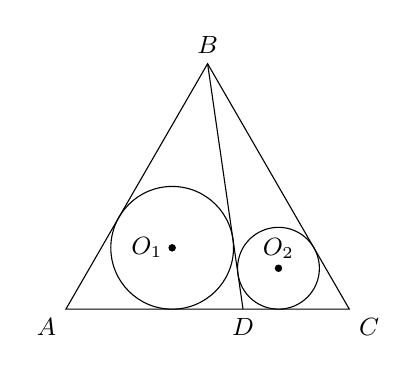
\begin{tikzpicture}[scale=0.45,font=\small]
\coordinate (A) at (0,0); \coordinate (C) at (8,0); \coordinate (B) at (4,6.928); \coordinate (D) at (5,0); \coordinate (O1) at (3,1.732); \coordinate (O2) at (6,1.155);
\draw (A)--(B)--(C)--cycle; \draw (B)--(D); \draw (O1) circle (1.732); \draw (O2) circle (1.155);
\fill (O1) circle (3pt); \fill (O2) circle (3pt);
\node[below left] at (A) {$A$}; \node[above] at (B) {$B$}; \node[below right] at (C) {$C$}; \node[below] at (D) {$D$}; \node[left] at (O1) {$O_1$}; \node[above] at (O2) {$O_2$};
\end{tikzpicture}}
\Opts{$5\sqrt3$}{$4\sqrt3$}{$\dfrac5{\sqrt3}$}{$\dfrac4{\sqrt3}$}}
\QQ{29}{Teng tomonli uçburçaklar rasmda körsatilgandek ustma-ust qöyilgan ($A$, $B$, $E$ — $ODC$ uçburçak tomonlarining örtalari, $F$ — $AD$ ning örtasi). $B$ nuqta koordinatasi $\left(6;\,2\sqrt3\right)$ bölsa, $\overrightarrow{CF}$ vektorning koordinatalari köpaytmasini toping.
\qfig{\begin{tikzpicture}[scale=0.42,font=\small]
\draw[-{Stealth[length=4pt]}] (-0.8,0)--(9.5,0) node[right] {$x$}; \draw[-{Stealth[length=4pt]}] (0,-0.8)--(0,8) node[left] {$y$};
\coordinate (O) at (0,0); \coordinate (C) at (8,0); \coordinate (D) at (4,6.928); \coordinate (A) at (2,3.464); \coordinate (B) at (6,3.464); \coordinate (E) at (4,0); \coordinate (F) at (3,5.196);
\draw (O)--(D)--(C); \draw (A)--(B)--(E)--cycle; \draw (C)--(F);
\draw ($(A)!0.5!(F)+(0.15,-0.09)$)--++(-0.3,0.18); \draw ($(F)!0.5!(D)+(0.15,-0.09)$)--++(-0.3,0.18);
\node[below left] at (O) {$O$}; \node[below] at (C) {$C$}; \node[above] at (D) {$D$}; \node[left] at (A) {$A$}; \node[right] at (B) {$B$}; \node[below] at (E) {$E$}; \node[left] at (F) {$F$};
\end{tikzpicture}}
\Opts{$-15\sqrt3$}{$-20\sqrt3$}{$-18\sqrt3$}{$-12\sqrt3$}}
\QQ{30}{Tekislikda yotmaydigan $A$ nuqtadan $AB$ va $AC$ oğmalar va $AH=5$ perpendikulyar tuşirilgan. $AB$ oğma va $AH$ perpendikulyar orasidagi burçak $30^\circ$, $AC$ oğma va $AH$ perpendikulyar orasidagi burçak $45^\circ$ bölsa, $B$ va $C$ nuqtalar orasidagi eng qisqa masofani toping.
\Opts{$5\left(\sqrt3-1\right)$}{$\dfrac{5\left(\sqrt3-1\right)}{\sqrt3}$}{$10\left(\sqrt3-1\right)$}{$10\left(\sqrt3+1\right)$}}
\QQ{31}{$A=\{24$ ning natural böluvçilari$\}$, $B=\{16$ ning natural böluvçilari$\}$ va $C=\{20$ ning natural böluvçilari$\}$ bölsa, $n(A)+n(B)-n(C)$ ni toping. Bu yerda $n(A)$ — $A$ töplamning elementlari soni.
\Opts{$5$}{$8$}{$9$}{$7$}}
\QQ{32}{Majlisda $30$ ta kişi qatnaşmoqda. Bu $30$ kişidan $8$ tasi ayol kişi. $30$ kişidan $3$ kişini tanlab oliş kerak. Barçaning tanlaniş imkoniyatlari teng. Tanlangan $3$ kişidan $2$ tasi erkak kişi, bittasi ayol kişi böliş ehtimolligini toping.
\Opts{$\dfrac{61}{145}$}{$\dfrac{66}{145}$}{$\dfrac{43}{145}$}{$\dfrac{47}{65}$}}
\QQ{33}{\Moslash{Apofemasi asos tekisligi bilan $60^\circ$ burçak hosil qiladigan töğri törtburçakli piramidaga şar içki çizilgan.}{A) $\dfrac\pi6$\par B) $\dfrac23$\par C) $\dfrac12$\par D) $\dfrac16$\par E) $\dfrac32$\par F) $\dfrac\pi9$}{Şar diametrining piramida balandligiga nisbatini toping.}{Şar sirti yuzining piramida yon sirti yuziga nisbatini toping.}{Şar hajmining piramida hajmiga nisbatini toping.}}
\QQ{36}{Tenglamani yeçing.
\[\lg x-\lg(x-2)=m\]
\AB{Tenglama yeçimga ega bölmaydigan $m$ ning eng katta qiymatini toping.}{Tenglama yeçimga ega böladigan $m$ ning barça qiymatlarini toping.}}
\QQ{37}{$a$ parametrli tenglama uçun
\[\sin^4x+\cos^4x=a\]
\AB{Tenglama yeçimga ega bölmaydigan $a$ ning eng kiçik natural qiymatini toping.}{Tenglama yeçimga ega böladigan $a$ ning eng katta butun maʼnosida tenglamaning $\left[-\dfrac\pi2;\,\dfrac\pi2\right]$ oraliqdagi yeçimlari sonini toping.}}
\QQ{38}{$f(x)$ funksiya uçun $f(x)+3f\left(\dfrac1x\right)=4x$ tenglik örinli bölsa,
\AB{$f(2)$ ni toping.}{$f(x)=0$ tenglik $x$ ning neçta qiymatida örinli?}}
\QQ{39}{$y=f(x)$ funksiya grafigi va unga $x=1$ nuqtada ötkazilgan $y=kx+l$ urinma berilgan.
\qfig{\begin{tikzpicture}[x=1.1cm,y=0.75cm,font=\small]
\draw[-{Stealth[length=4pt]}] (-0.6,0)--(3.6,0) node[right] {$x$}; \draw[-{Stealth[length=4pt]}] (0,-1.9)--(0,3.6) node[left] {$y$};
\draw[thick,domain=-0.1:2.25,samples=60] plot (\x,{2-(\x-1)-1.5*(\x-1)*(\x-1)}); \draw (-0.3,3.3)--(3.3,-0.3);
\draw[dashed] (0,2)--(1,2)--(1,0); \fill (1,2) circle (2pt);
\node[left] at (0,2) {$2$}; \node[below] at (1,0) {$1$}; \node[below] at (3,0) {$3$};
\node[right] at (0.2,3.1) {$y=kx+l$}; \node[right] at (2.15,-1.7) {$y=f(x)$};
\end{tikzpicture}}
\AB{$f'(1)$ ni toping.}{$h(x)=\left(x^3-2x^2+x+3\right)\cdot f(x)$ bölsa, $h'(1)$ ni toping.}}
\QQ{40}{$y=2$ va $y=\dfrac{x^2}2$ funksiyalar berilgan.
\AB{Funksiyalar grafiklari bilan çegaralangan soha yuzini toping.}{Şu sohani $Oy$ öqi atrofida aylantirişdan hosil bölgan jism hajmini toping.}}
\QQ{41}{$MN$ diametrli yarim aylanada yuzi $20$ ga teng bölgan $ABC$ töğri burçakli uçburçak ($\angle C=90^\circ$, $\angle ABC=15^\circ$) berilgan: $A$ va $B$ yarim aylanada, $AB\parallel MN$, $C$ nuqta $MN$ da yotadi. $O$ nuqta aylananing markazi.
\qfig{\begin{tikzpicture}[scale=0.32,font=\small]
\coordinate (O) at (0,0); \coordinate (M) at (-7.071,0); \coordinate (N) at (7.071,0); \coordinate (A) at (-6.325,3.162); \coordinate (B) at (6.325,3.162); \coordinate (C) at (-5.478,0);
\draw (N) arc (0:180:7.071); \draw (M)--(N); \draw (A)--(B)--(C)--cycle; \fill (O) circle (4pt);
\draw ($(C)!0.6cm!(A)$)--($(C)!0.6cm!(A)+(C)!0.6cm!(B)-(C)$)--($(C)!0.6cm!(B)$);
\draw (B)+(180:1.6) arc (180:195:1.6); \node at (3.9,2.75) {\scriptsize$15^\circ$};
\node[above left] at (A) {$A$}; \node[above right] at (B) {$B$}; \node[below] at (C) {$C$}; \node[below] at (O) {$O$}; \node[below left] at (M) {$M$}; \node[below right] at (N) {$N$};
\end{tikzpicture}}
\AB{$|AB|$ ni toping.}{$O$ va $N$ nuqtalar orasidagi masofani toping.}}
\QQ{42}{Quyidagi çizmada uçta bir xil kvadrat berilgan: $ABKM$ töğri törtburçak ikki kvadratdan iborat, $CDEF$ kvadratning $CF$ tomoni $BK$ da yotadi va uning örtasi pastki kvadratlarning umumiy uçi.
\qfig{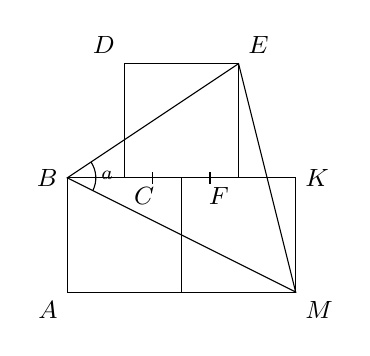
\begin{tikzpicture}[scale=1.45,font=\small]
\coordinate (A) at (0,0); \coordinate (M) at (2,0); \coordinate (K) at (2,1); \coordinate (B) at (0,1); \coordinate (C) at (0.5,1); \coordinate (F) at (1.5,1); \coordinate (D) at (0.5,2); \coordinate (E) at (1.5,2);
\draw (A)--(M)--(K)--(B)--cycle; \draw (1,0)--(1,1); \draw (C)--(D)--(E)--(F);
\draw (B)--(E)--(M)--cycle;
\draw (0.75,0.95)--(0.75,1.05); \draw (1.25,0.95)--(1.25,1.05);
\draw (B)+(-26.57:0.25) arc (-26.57:33.69:0.25); \node at (0.35,1.02) {\scriptsize$a$};
\node[below left] at (A) {$A$}; \node[below right] at (M) {$M$}; \node[right] at (K) {$K$}; \node[left] at (B) {$B$}; \node[below right] at (C) {$C$}; \node[below left] at (F) {$F$}; \node[above left] at (D) {$D$}; \node[above right] at (E) {$E$};
\end{tikzpicture}}
\AB{$a$ burçakning kosinusini toping.}{Kvadratning tomoni $6$ ga teng bölsa, $BEM$ uçburçakning yuzini toping.}}
\QQ{43}{Quyidagi çizmada $ABCDEF$ muntazam oltiburçak berilgan, $G$ — $AB$ tomonning örtasi.
\qfig{\begin{tikzpicture}[scale=1.25,font=\small]
\coordinate (C) at (0,1); \coordinate (D) at (0.866,0.5); \coordinate (E) at (0.866,-0.5); \coordinate (F) at (0,-1); \coordinate (A) at (-0.866,-0.5); \coordinate (B) at (-0.866,0.5); \coordinate (G) at (-0.866,0);
\fill[qfill] (G)--(C)--(D)--cycle;
\draw (A)--(B)--(C)--(D)--(E)--(F)--cycle; \draw (G)--(C)--(D)--cycle;
\draw (-0.926,0.25)--(-0.806,0.25); \draw (-0.926,-0.25)--(-0.806,-0.25);
\node[above] at (C) {$C$}; \node[right] at (D) {$D$}; \node[right] at (E) {$E$}; \node[below] at (F) {$F$}; \node[left] at (A) {$A$}; \node[left] at (B) {$B$}; \node[left] at (G) {$G$};
\end{tikzpicture}}
\AB{Böyalgan soha yuzining böyalmagan soha yuziga nisbatini toping.}{Oltiburçak tomoni $8$ ga teng bölsa, $DGC$ uçburçakning yuzini toping.}}
\QQ{44}{Asosining radiusi $3$ ga teng bölgan konusga eng katta yon sirtga ega bölgan silindr içki çizilgan. Konusning yon sirti yoyilmasi yarim doiradan iborat.
\AB{Konus yasovçisini toping.}{Silindrning yon sirti yuzini toping.}}
\QQ{45}{Eni $12$ cm bölgan töğri törtburçakli tunuka berilgan.
\qfig{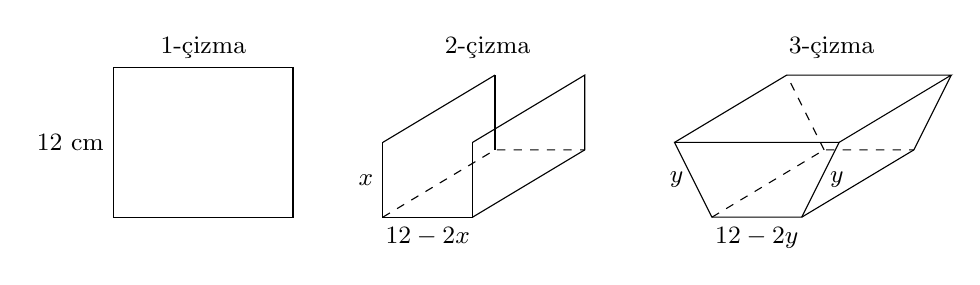
\begin{tikzpicture}[scale=0.95,font=\small]
\draw (0,0) rectangle (2.4,2); \node[left] at (0,1) {$12$ cm}; \node[above] at (1.2,2) {1-çizma};
\begin{scope}[xshift=3.6cm]
\draw (0,1)--(0,0)--(1.2,0)--(1.2,1); \draw (0,1)--(1.5,1.9); \draw (1.2,1)--(2.7,1.9)--(2.7,0.9)--(1.2,0); \draw[dashed] (0,0)--(1.5,0.9)--(2.7,0.9); \draw (1.5,1.9)--(1.5,0.9);
\node[left] at (0,0.5) {$x$}; \node[below] at (0.6,0) {$12-2x$}; \node[above] at (1.4,2) {2-çizma};
\end{scope}
\begin{scope}[xshift=8cm]
\draw (-0.5,1)--(0,0)--(1.2,0)--(1.7,1)--cycle; \draw (-0.5,1)--(1,1.9)--(3.2,1.9)--(1.7,1); \draw (3.2,1.9)--(2.7,0.9)--(1.2,0); \draw[dashed] (0,0)--(1.5,0.9)--(2.7,0.9); \draw[dashed] (1.5,0.9)--(1,1.9);
\node[left] at (-0.25,0.5) {$y$}; \node[right] at (1.45,0.5) {$y$}; \node[below] at (0.6,0) {$12-2y$}; \node[above] at (1.6,2) {3-çizma};
\end{scope}
\end{tikzpicture}}
\AB{Tunuka ikki çetidan $x$ cm dan qayrilib, eng katta köndalang kesim yuzasiga ega bölgan tarnov hosil qilingan. $x$ ni toping (cm).}{Tunuka ikki çetidan $y$ cm qayrilib, eng katta köndalang kesimli teng yonli trapetsiya şaklidagi tarnov hosil qilindi. Köndalang kesim yuzini toping (cm$^2$).}}
\Javoblar{B A C C B B C B A D C C D D D A D B C B D A C A A D B C A B D B B A F}{%
\OK{36}{$0$}{$(0;\,\infty)$}\OK{37}{$2$}{$3$}\OK{38}{$-\dfrac14$}{$2$}\OK{39}{$-1$}{$-3$}\OK{40}{$\dfrac{16}3$}{$4\pi$}%
\OK{41}{$4\sqrt{10}$}{$5\sqrt2$}\OK{42}{$\dfrac4{\sqrt{65}}$}{$63$}\OK{43}{$\dfrac13$}{$24\sqrt3$}\OK{44}{$6$}{$\dfrac{9\sqrt3}2\pi$}\OK{45}{$3$}{$12\sqrt3$}}
